\chapter{Reconstruction}
\label{sec:reconstruction}
A series of reconstruction algorithms are run over all events that pass data cleaning.
These algorithms estimate the position, time, direction, and energy of the event.
All events are reconstructed under the hypothesis that the PMT hits are from Cherenkov radiation
produced by a single electron.
Additionally, the reconstruction algorithms use only the hits in a prompt time window to ensure only light
that travelled directly from the event origin is used,
though each algorithm defines differently window is used.
Only hits that are from well calibrated, online PMTs and detector channels are used.
%The reconstruction algorithms used in this analysis are all algorithms that were developed for SNO\@.
%Since having a light-water vs heavy-water target has small and easily accounted for effects on the emission of Cherenkov radiation inside the AV, these algorithms perform effectively for the SNO+ water phase as they did for SNO\@.
The same reconstruction algorithms are used on both simulated and detected events.

The direction ($\vec{d}$), time ($t_{0}$), and position ($\vec{p}$) are determined by performing a likelihood
fit to the time and position of PMT hits.
Only hits within a $100$\,ns window centered around the mode of the raw hit time
distribution are used.
The algorithm evaluates the likelihood of a hypothesized event position and time by
calculating the time residual for each hit PMT,
\begin{equation}
\label{eqn:tres}
t_{res} = t_{PMT} - t_{transit} - t_{0}\text{.}
\end{equation}
The transit time is calculated by considering the distance the photon would
traverse in inner volume water, the external water, and inside the AV acrylic, as
it travels from the hypothesized position to the PMT, accounting for refractions
at boundaries.
From those distances the transit time is simply calculated as
\begin{equation}
t_{transit} = \frac{d_{\mathrm{AV}}}{v_{\mathrm{AV}}} + \frac{(d_{\mathrm{inner}} + d_{\mathrm{external}})}{v_{\mathrm{water}}}\text{,}
\end{equation}
the group-velocity for 400\,nm light is used as the velocity.

\begin{figure}[htbp]
\centering
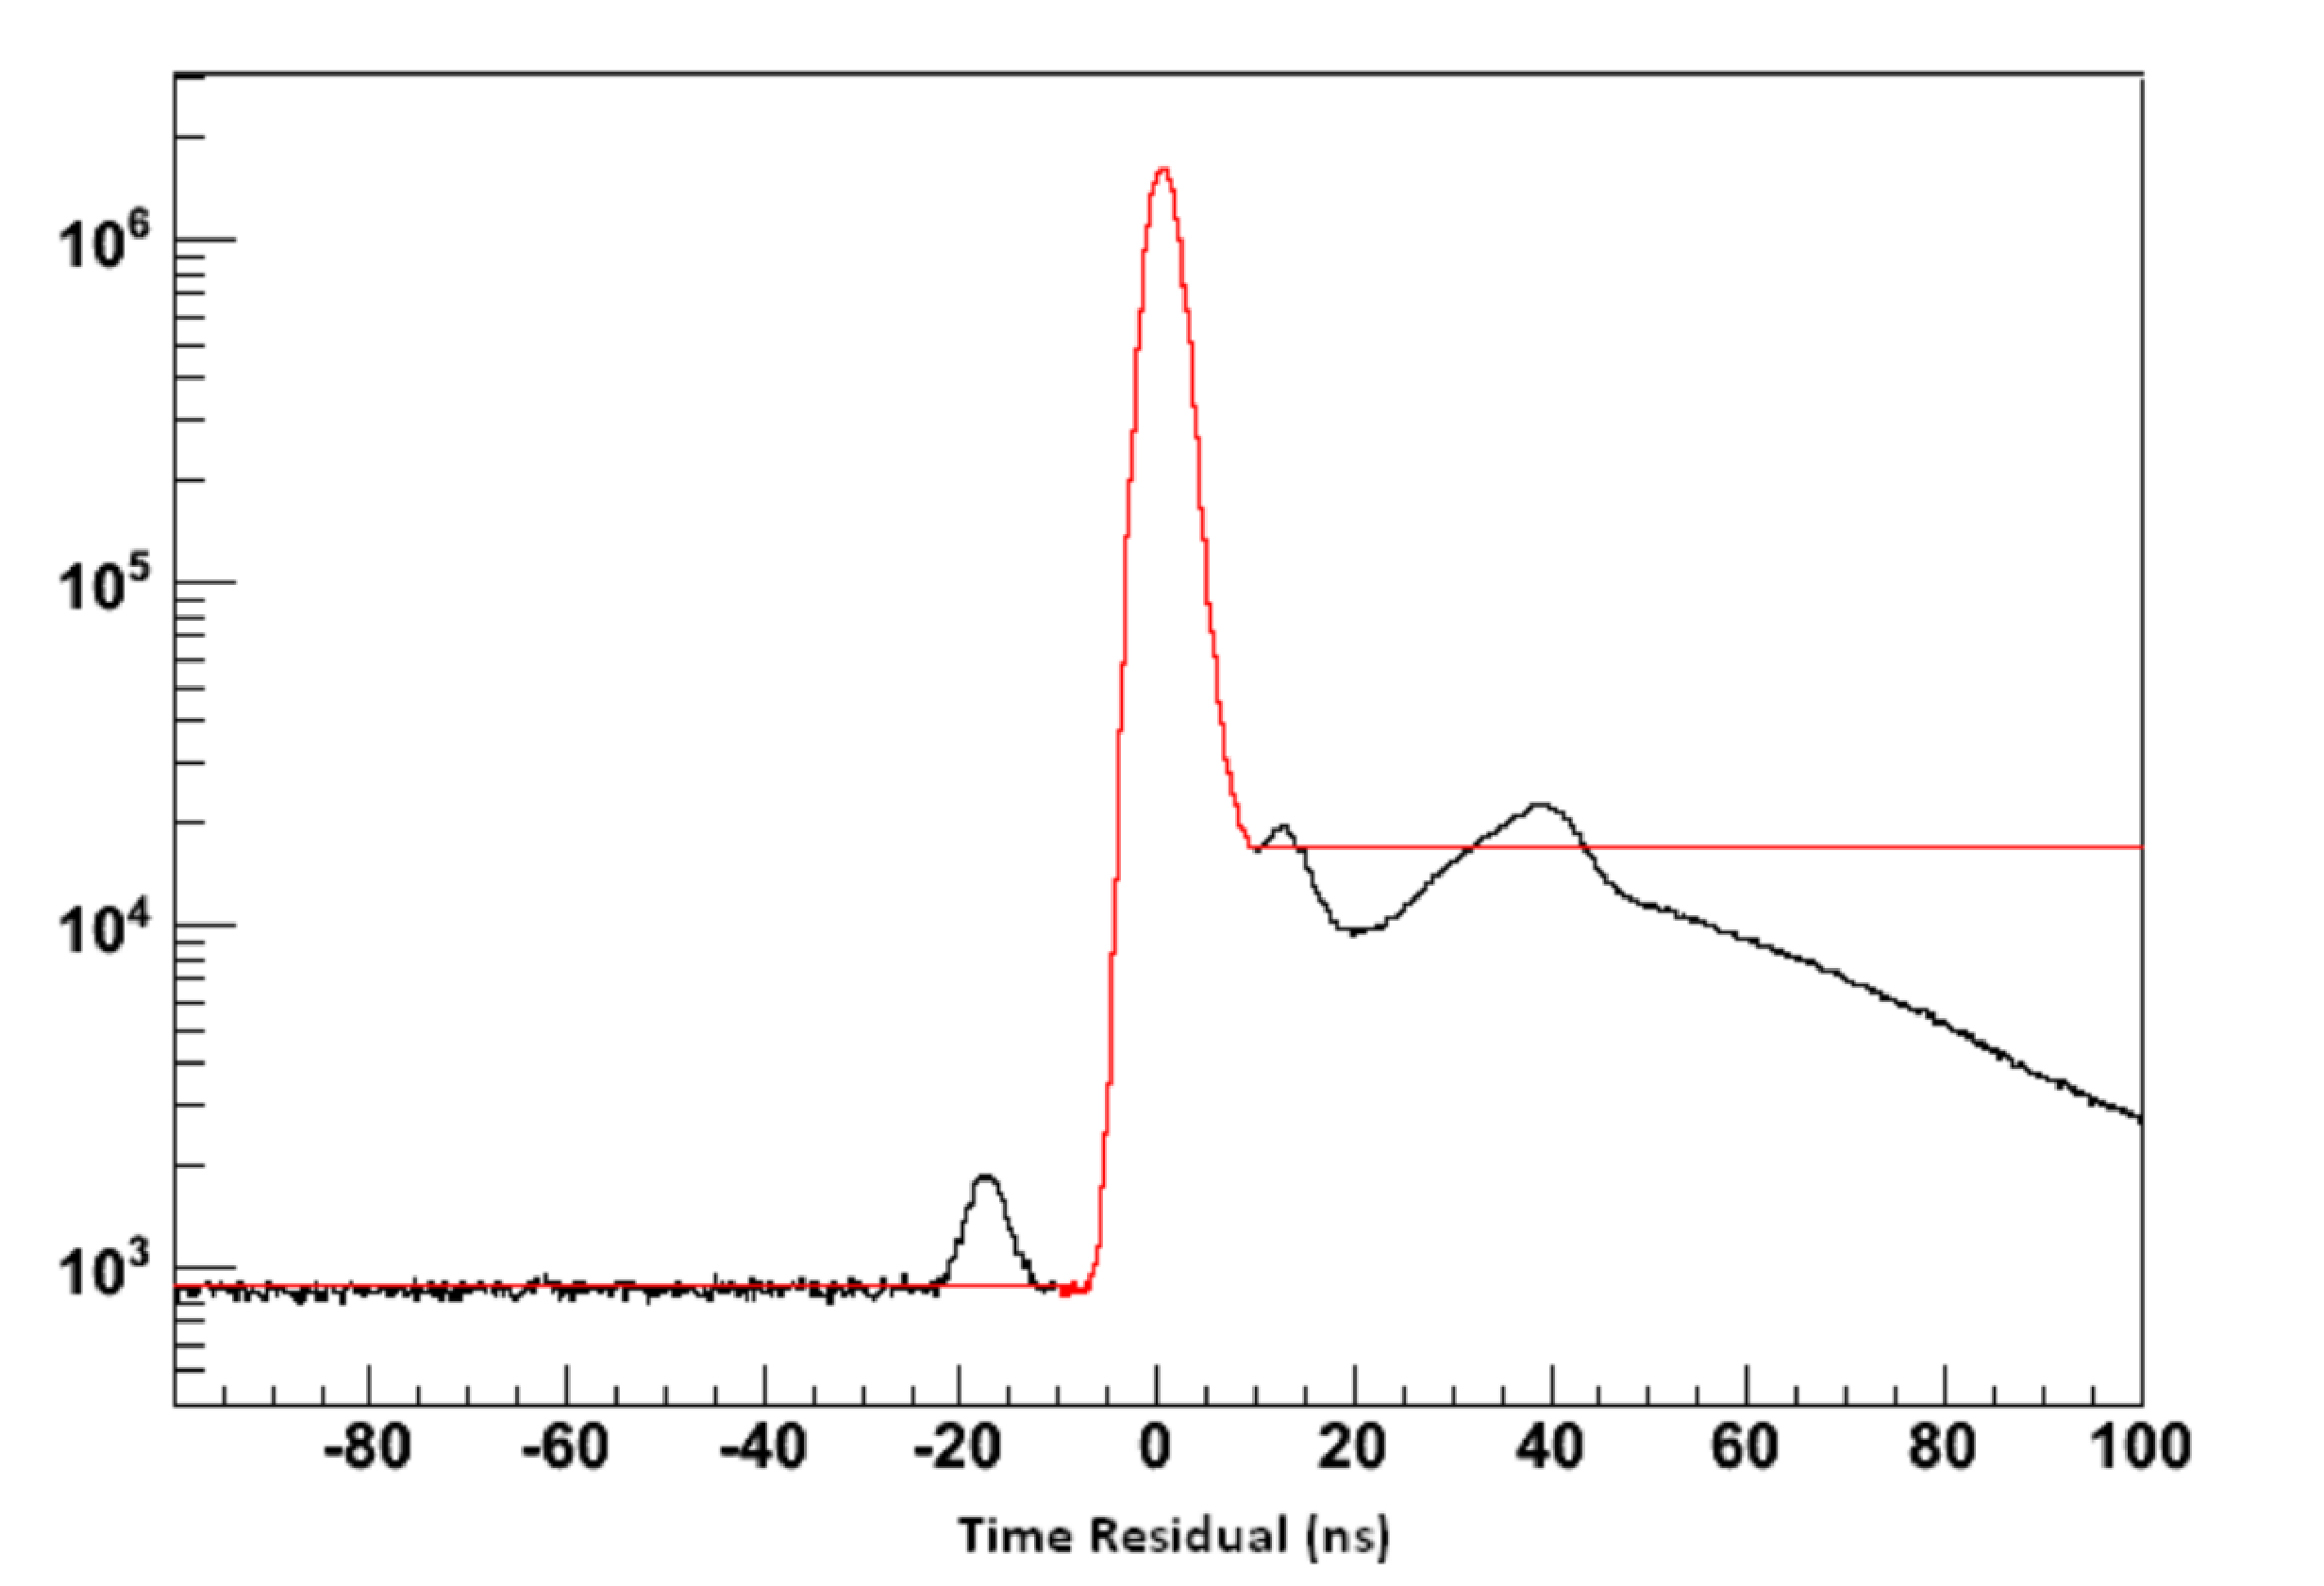
\includegraphics[width=0.78\textwidth]{tres_dist}
\caption[Simulated Distribution of $t_{\mathrm{res}}$]{
(black) Distribution of time residuals for simulated 6\,MeV electrons. (red) Simplified
timing distribution used for reconstruction. Figure from~\citep{richie_thesis}.}
\label{fig:tres_dist}
\end{figure}

The PDF for $t_{\mathrm{res}}$, $P(t_{\mathrm{res}})$, is determined from prior simulation,
Fig.~\ref{fig:tres_dist} shows this PDF compared to a full timing simulation.
The position and time that minimize the quantity
\begin{equation}
\sum_{i=0}^{N_{PMT}} P(t_{res}) % TODO need to refactor this to include the index i
\end{equation}
is used as the event position and time.

The direction is determined by evaluating $\theta_{\mathrm{PMT}}$ for each hit where
$\theta_{\mathrm{PMT}}$ is defined by,
\begin{equation}
    \cos\theta_{\mathrm{PMT}} = \vec{d}\cdot\left(\vec{p}_{PMT} - \vec{p}\right)\text{.}
\end{equation}
The likelihood, $P(\theta_{\mathrm{PMT}})$, is determined from a prior simulation of
6\,MeV electrons at the center of the detector, Fig~\ref{fig:rat_angle_pdf} shows
this PDF\@. %That PDF is modified by a correction to account for the fact that PMTs nearer to the event vertex are more likely to be hit.
The direction that minimizes
\begin{equation}
\sum_{i=0}^{N_{PMT}} P(\theta_{\mathrm{PMT}})
\end{equation}
is used as the reconstructed event direction.

\begin{figure}[htbp]
\centering
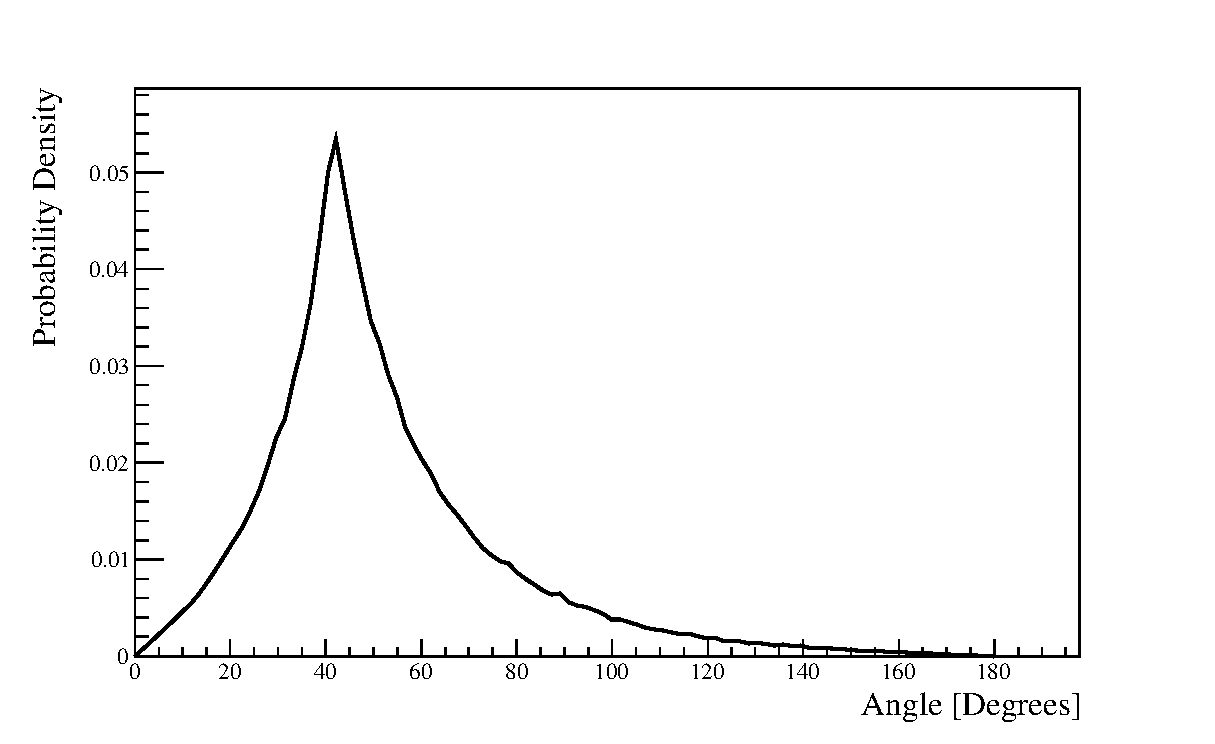
\includegraphics[width=0.78\textwidth]{rat_angle_pdf}
\caption[RAT PDF for Direction Fit]{The PDF used by RAT when evaluating the
likelihood of a hypothesized direction.  The peak at approximately $40^{\circ}$
corresponds to the Cherenkov cone opening angle.}
\label{fig:rat_angle_pdf}
\end{figure}

The kinetic energy of the event is determined after
the event position, time and direction are determined.
The position and time are used to determine the number of PMT
hits that occurred in a prompt 18\,ns window.
Then the number of photons that would most likely produce
that number of PMT hits is estimated using a combination of
analytic calculation and PDFs from prior simulation.
A look up table is used to estimate the most likely electron
kinetic energy that would produce the determined number of photons.
This method of energy reconstruction is called ``EnergyRSP'', which stands
simply for Energy Response.

\begin{figure}[htbp]
\centering
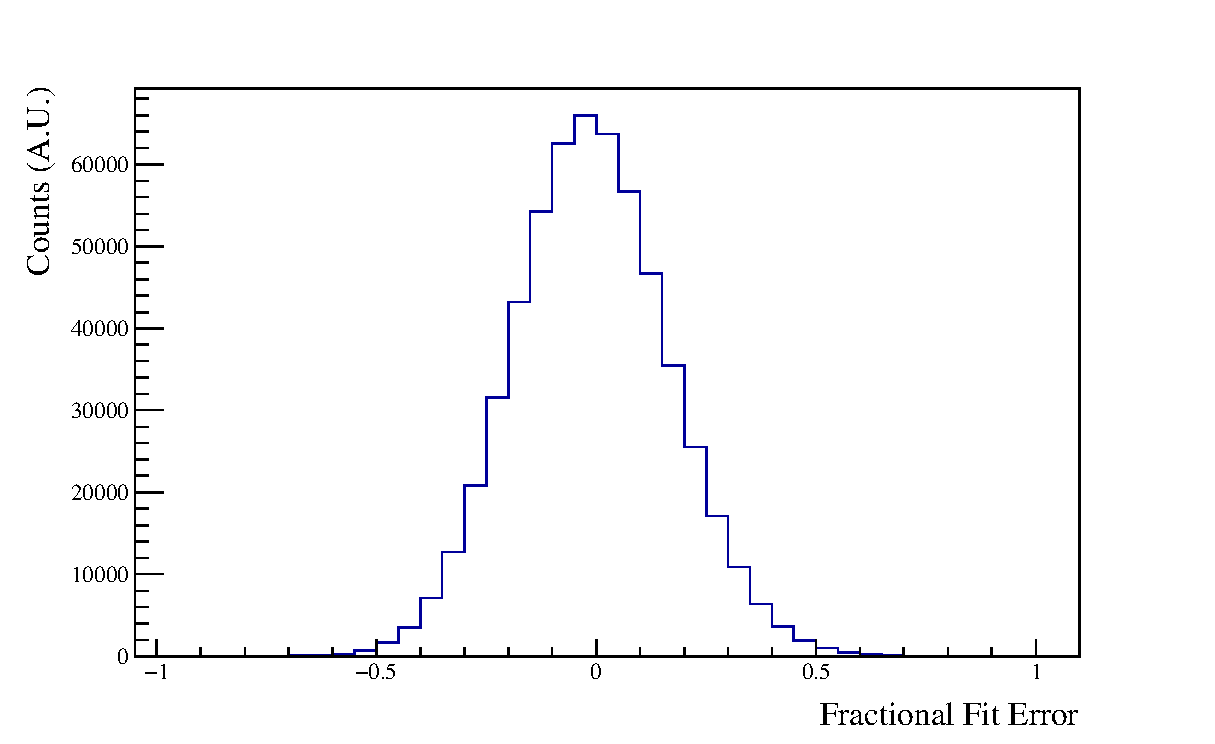
\includegraphics[width=0.78\textwidth]{fit_residual_nofit}
\caption[EnergyRSP Fit Residuals]{Fractional error of fitted energy   for solar $\nu_{\mathrm{e}}$ events
with simulated energy above 5\,MeV.
}
\label{fig:mc_fit_residuals}
\end{figure}
The uncertainty in the energy fit is dominated by the uncertainty
introduced by the photon-statistics associated with Cherenkov radiation.
For electrons the number of detected photons per MeV kinetic energy is approximately 7.
Meaning a 5\,MeV electron event will on average produce 35 PMT hits with
one-sigma statistical fluctuations of roughly $\sqrt{35} \approx 5.9$, or about 17\%.
Figure~\ref{fig:mc_fit_residuals} shows the residuals for fit results on MC simulated solar $\nu_{e}$ events.

%An error was found in the calculation of the number of Cherenkov photons expected for an electron of a given energy.
